\documentclass{article}
\usepackage[utf8]{inputenc}
\usepackage{graphicx}
\usepackage{listings}

\lstset{language=SQL}

\title{CS 313: Assignment 3}
\author{Om Patil}
\date{August 2021}

\begin{document}

\maketitle

\section{}
\begin{lstlisting}
create user 'lab3'@'localhost' identified by 'iitdh';
create database lab3;
grant all privileges on lab3.* to 'lab3'@'localhost';
\end{lstlisting}
\begin{center}  
    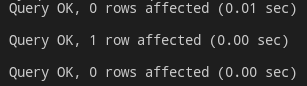
\includegraphics[scale=0.6]{1.png}
\end{center}

\section{}
\begin{lstlisting}
use lab3;

create table part (
    part_no int,
    part_name varchar(25),
    color varchar(15),
    weight int,
    primary key (part_no)
);

create table supplier (
    supplier_no int,
    sup_name varchar(25),
    city varchar(25),
    bank varchar(25),
    primary key (supplier_no)
);

create table shipment (
    shipment_no int,
    part_no int,
    supplier_no int,
    date date,
    quantity int,
    price int,
    primary key (shipment_no),
    foreign key (part_no) references part(part_no),
    foreign key (supplier_no) references supplier(supplier_no)
    );
\end{lstlisting}
\begin{center}
    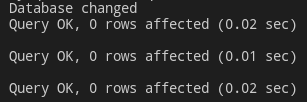
\includegraphics[scale=0.6]{2.png}
\end{center}

\section{}
\begin{lstlisting}
insert into part values (1, 'screw', 'silver', 12);
insert into supplier values (1, 'Singh Screw Co.', 'Delhi', 'SBI');
insert into shipment values (1, 1, 1, '2022-05-15', 100, 10);
\end{lstlisting}
\begin{center}
    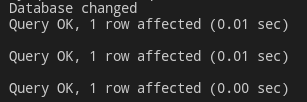
\includegraphics[scale=0.6]{3.png}
\end{center}

\section{}
\begin{lstlisting}
-- Parts
insert into part values (2, 'nut', 'black', 16);
insert into part values (3, 'bolt', 'red', 17);

-- Suppliers
insert into supplier values (2, 'Baburao & Sons', 'Mumbai', 'ICICI');
insert into supplier values (3, 'Rajesh Hardware', 'Chennai', 'HDFC');

-- Shipments
insert into shipment values (2, 1, 2, '2022-05-21', 200, 20);
insert into shipment values (3, 1, 1, '2021-06-13', 300, 30);
insert into shipment values (4, 1, 1, '2018-11-04', 400, 25);
insert into shipment values (5, 2, 1, '2003-02-26', 250, 15);
insert into shipment values (6, 2, 2, '2020-05-18', 650, 10);
insert into shipment values (7, 2, 2, '2019-12-05', 100, 20);
insert into shipment values (8, 2, 2, '2020-03-14', 200, 17);
insert into shipment values (9, 3, 1, '2012-12-30', 130, 20);
insert into shipment values (10, 3, 1, '2019-01-01', 150, 25);
insert into shipment values (11, 3, 1, '2014-11-26', 455, 12);
insert into shipment values (12, 3, 1, '2021-02-22', 120, 20);

-- Display Part table
select * from part;

-- Display Supplier table
select * from supplier;

-- Display Shipment table
select * from shipment;
\end{lstlisting}
\begin{center}
    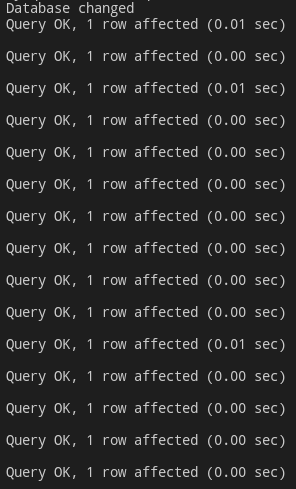
\includegraphics[scale=0.6]{4i.png}
    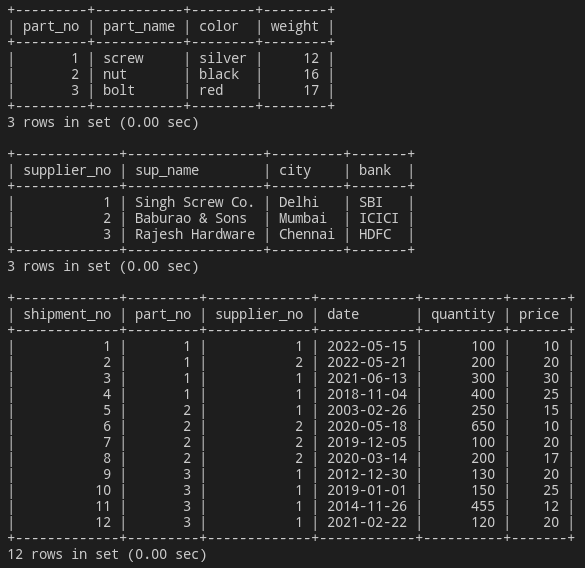
\includegraphics[scale=0.6]{4ii.png}
\end{center}

\section{}
\begin{lstlisting}
-- a
select distinct sup_name 
from supplier
natural join shipment
natural join part
where color = 'red';
\end{lstlisting}
\begin{center}
    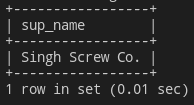
\includegraphics[scale=0.6]{5a.png}
\end{center}

\begin{lstlisting}
-- b
select sup_name, sum(quantity * price) as total
from shipment
natural join supplier
group by sup_name;
\end{lstlisting}
\begin{center}
    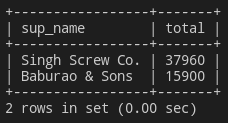
\includegraphics[scale=0.6]{5b.png}
\end{center}

\begin{lstlisting}
-- c
select distinct sup_name 
from shipment
natural join supplier;
\end{lstlisting}
\begin{center}
    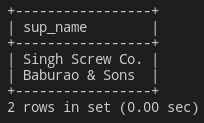
\includegraphics[scale=0.6]{5c.png}
\end{center}

\end{document}